\documentclass[11pt]{article}
\usepackage[margin=0.95in]{geometry}
\usepackage{amsmath,amssymb,amsthm,mathtools}
\usepackage{booktabs,array,graphicx,xcolor,enumitem,microtype}
\usepackage[colorlinks=true,linkcolor=blue,citecolor=blue,urlcolor=blue]{hyperref}

\theoremstyle{plain}
\newtheorem{theorem}{Theorem}[section]
\newtheorem{proposition}[theorem]{Proposition}
\newtheorem{lemma}[theorem]{Lemma}
\newtheorem{corollary}[theorem]{Corollary}
\theoremstyle{definition}
\newtheorem{definition}[theorem]{Definition}
\newtheorem{assumption}[theorem]{Assumption}
\theoremstyle{remark}
\newtheorem{remark}[theorem]{Remark}

\newcommand{\E}{\mathbb{E}}
\newcommand{\Prob}{\mathbb{P}}
\newcommand{\Var}{\mathrm{Var}}
\newcommand{\Cov}{\mathrm{Cov}}
\newcommand{\Corr}{\mathrm{Corr}}
\newcommand{\tvd}{\mathrm{TV}}
\newcommand{\R}{\mathbb{R}}

\title{\textbf{Redundancy-Balanced Spectral Peer TVD-MI:}\\
Complete Mathematical Derivations, Lean~4 Formalization,\\
and Real-LLM Falsification \& Recovery}
\author{Project: \texttt{brando90/tvdmi-judge-asymptotics} (Experiment~13, 11-21-2026)}
\date{Date: 11-21-2026 \quad(\emph{As of 11-21-2026 19:06 PST})}

\newcommand{\lident}[1]{{\small\texttt{#1}}}

\begin{document}
\maketitle

\noindent\textbf{Provenance.} Formal proofs are machine-checked in
\lident{TvdmiJudge/NewTheory.lean} inside\\
\lident{experiments/00\_\allowbreak lean\_\allowbreak formalization/lean/}
(\texttt{Lean v4.29.0}, \texttt{lake build}, 3,288 jobs, zero \texttt{sorry},
standard kernel axioms \texttt{[propext, Classical.choice, Quot.sound]}).
Empirical validation runs via
\lident{run\_\allowbreak real\_\allowbreak llm\_\allowbreak and\_\allowbreak theory\_\allowbreak suite.py} inside\\
\lident{experiments/13\_\allowbreak ...\_\allowbreak 21Nov2026/}
(\texttt{seed=42}, single-process Python 3.11, 5-fold cluster-held-out evaluation
on public \textsc{SummEval} and \textsc{LMSYS MT-Bench} plus 500-repetition Monte
Carlo simulations).

\section{What These Results Show and Do Not Show (Explicit Limits)}

\begin{center}
\fbox{\parbox{0.96\textwidth}{%
\textbf{Scope \& Metric Boundaries (As of 11-21-2026):}
\begin{enumerate}[leftmargin=1.4em,itemsep=3pt]
  \item \textbf{Unconditional TVD-MI measures dependence, not truth:}
    $\tvd(P_{X,Y}, P_X \otimes P_Y)$ cannot distinguish task execution from
    invertible prompt transformations $Y = f(X)$ (Theorem~\ref{thm:inj}) or
    global label inversions $Y = 1 - Z^\star$. On \textsc{SummEval}, verbatim
    article copying achieves prompt--response TF-IDF TVD-MI $0.4851$, exceeding
    every real summarization model ($\le 0.3277$).
  \item \textbf{Rank consistency vs.\ absolute Likert severity:}
    Double-centering cancels arbitrary additive prompt difficulty $a(x)$ and
    verbosity/leniency $b(y)$ exactly (Theorem~\ref{thm:dc}), isolating rank
    order. Without a human calibration anchor, \texttt{RB-Spec TVD-MI} attains
    high item Spearman ($+0.689$) and consistency ($\mathrm{ICC(C,1)}=0.688$)
    while retaining G-Eval's harsh mean offset ($-1.111$ vs.\ human $4.131$,
    $\mathrm{ICC(A,1)}=0.351$).
  \item \textbf{Hierarchical clone-hijacking falsification vs.\ $1/F$ recovery:}
    When $F$ judge families emit unbalanced clone counts $K_1,\dots,K_F$, uniform
    averaging converges to a cloned weak family's floor $\tau_1^2$ and can invert
    adversarial majority signs. \texttt{RB-Spec TVD-MI} restores $O(1/F)$ scaling
    and effective-family breakdown $\delta_{\mathrm{fam}} < 1/2$, provided fewer
    than half of independent families are adversarial and a latent shared confound
    $W$ does not reverse more than half of all distinct families.
\end{enumerate}}}
\end{center}

\section{Finite-Alphabet Variational Duality and Injection Blindness}

Let $\mathcal{U}$ and $\mathcal{V}$ be finite alphabets of prompts $X$ and
candidate outputs $Y$. Let $P_X$ denote the prompt probability mass function
($P_X(x) \ge 0$, $\sum_x P_X(x) = 1$).

\begin{theorem}[Finite-PMF variational duality]
\noindent\textit{Lean 4:} \lident{finite\_\allowbreak tvd\_\allowbreak variational\_\allowbreak le},
\lident{finite\_\allowbreak tvd\_\allowbreak variational\_\allowbreak eq}.\par\medskip
Let $p, q : \mathcal{A} \to \R$ satisfy $\sum_{x \in \mathcal{A}} p(x) = \sum_{x \in \mathcal{A}} q(x)$.
For any bounded witness critic $h : \mathcal{A} \to [0,1]$,
\[
  \sum_{x \in \mathcal{A}} p(x)h(x) - \sum_{x \in \mathcal{A}} q(x)h(x)
  \le \frac{1}{2}\sum_{x \in \mathcal{A}} |p(x) - q(x)|,
\]
with exact equality attained by the Scheff\'e critic $h^\star(x) := \mathbf{1}\{p(x) \ge q(x)\}$.
\end{theorem}
\begin{proof}
Define $d(x) := p(x) - q(x)$, so $\sum_x d(x) = 0$. For every $x \in \mathcal{A}$,
the real identity $|d(x)| = 2\max(d(x), 0) - d(x)$ holds by case analysis on
$\mathrm{sign}(d(x))$. Summing over $x \in \mathcal{A}$ gives
$\sum_x |d(x)| = 2\sum_x \max(d(x),0) - \sum_x d(x) = 2\sum_x \max(d(x),0)$.
Furthermore, since $h(x) \in [0,1]$, if $d(x) \ge 0$ then $d(x)h(x) \le d(x) = \max(d(x),0)$,
and if $d(x) < 0$ then $d(x)h(x) \le 0 = \max(d(x),0)$. Summing gives
$\sum_x d(x)h(x) \le \sum_x \max(d(x),0) = \frac{1}{2}\sum_x |d(x)|$, with
equality at $h^\star(x) = \mathbf{1}\{d(x) \ge 0\}$ because $d(x)h^\star(x) = \max(d(x),0)$.
\end{proof}

\begin{theorem}[Injection blindness; Lean: \texttt{injection\_tvd\_blindness}]
\label{thm:inj}
Let $f : \mathcal{U} \to \mathcal{V}$ be any injective map and set $Y = f(X)$,
so $P_{XY}(x,y) = P_X(x)\mathbf{1}\{y = f(x)\}$ and $P_Y(y) = \sum_{x'} P_X(x')\mathbf{1}\{f(x') = y\}$.
Then
\begin{equation}
\boxed{\;
\tvd\!\big(P_{X,f(X)}, P_X \otimes P_{f(X)}\big)
= \frac{1}{2}\sum_{x\in\mathcal{U}}\sum_{y\in\mathcal{V}} \big|P_{XY}(x,y) - P_X(x)P_Y(y)\big|
= 1 - \sum_{x\in\mathcal{U}} P_X(x)^2.\;}
\end{equation}
\end{theorem}
\begin{proof}
Because $f$ is injective, $f(x') = f(x) \iff x' = x$, so $P_Y(f(x)) = P_X(x)$,
and summing $P_Y(y)$ over $y \in \mathcal{V}$ gives $\sum_x P_X(x) = 1$. Fix $x$:
\begin{itemize}[leftmargin=*,itemsep=2pt]
  \item Diagonal term $y = f(x)$: since $0 \le P_X(x) \le 1$, $|P_X(x) - P_X(x)^2| = P_X(x) - P_X(x)^2$.
  \item Off-diagonal sum $y \neq f(x)$: $\sum_{y \neq f(x)} |0 - P_X(x)P_Y(y)| = P_X(x)\sum_{y \neq f(x)} P_Y(y) = P_X(x)(1 - P_X(x)) = P_X(x) - P_X(x)^2$.
\end{itemize}
Adding both gives $2(P_X(x) - P_X(x)^2)$ per $x$; summing over $x$ and multiplying by $1/2$ yields
$1 - \sum_x P_X(x)^2$. Notice $h$ ignores whether $f$ solves the task: verbatim
copying $Y=X$ saturates near $1$ on diverse prompts.
\end{proof}

\section{Double-Centering Invariance and Oriented Conditional Peer TVD-MI}

\begin{theorem}[Double-centering additive shift invariance]
\label{thm:dc}
\noindent\textit{Lean 4:} \lident{tvdmi\_\allowbreak double\_\allowbreak centering\_\allowbreak invariance}.\par\medskip
Let $P_{XY}$ have marginals $P_X(x) = \sum_y P_{XY}(x,y)$ and $P_Y(y) = \sum_x P_{XY}(x,y)$
with $\sum_x P_X(x) = \sum_y P_Y(y) = 1$. For any additive prompt-difficulty bias
$a : \mathcal{U} \to \R$, additive response-verbosity/leniency bias $b : \mathcal{V} \to \R$,
and interaction critic $\psi(x,y)$ scaled by $\gamma \in \R$,
\begin{equation}
\boxed{\;
h(x,y) = a(x) + b(y) + \gamma\,\psi(x,y)
\;\Longrightarrow\;
\E_{P_{XY}}[h] - \E_{P_X \otimes P_Y}[h] = \gamma\Big(\E_{P_{XY}}[\psi] - \E_{P_X \otimes P_Y}[\psi]\Big).\;}
\end{equation}
\end{theorem}
\begin{proof}
By marginal compatibility,
\[
  \sum_{x,y} P_{XY}(x,y) a(x) = \sum_x P_X(x) a(x) = \sum_x P_X(x)a(x)\sum_y P_Y(y) = \sum_{x,y} P_X(x)P_Y(y)a(x),
\]
and exchanging summation order yields $\sum_{x,y} P_{XY}(x,y)b(y) = \sum_y P_Y(y)b(y) = \sum_{x,y} P_X(x)P_Y(y)b(y)$.
Thus additive prompt and output offsets cancel identically. By contrast, raw
score means shift by $\E[a(X)] + \E[b(Y)]$ (confirmed on \textsc{SummEval}: raw
max shift $1.5464$ vs.\ double-centered shift $4.00\times 10^{-15}$).
\end{proof}

\begin{proposition}[Oriented conditional peer TVD-MI]
\noindent\textit{Lean 4:} \lident{oriented\_\allowbreak peer\_\allowbreak strict\_\allowbreak mono},
\lident{oriented\_\allowbreak peer\_\allowbreak rejects\_\allowbreak inverter}.\par\medskip
Let $Z^\star \in \{0,1\}$ denote latent item truth, $W_j \in \{0,1\}$ a
conditionally independent peer judge ($W_j \perp Y_c \mid Z^\star$) with
symmetric accuracy $q_j = \Prob(W_j = Z^\star \mid Z^\star)$, and
$Y_c \in \{0,1\}$ a candidate output with symmetric accuracy
$p_c = \Prob(Y_c = Z^\star \mid Z^\star)$ under independent copy
$\widetilde{Y}_c \sim P_{Y_c}$. Defining the oriented contrast
\[
  \Delta^{\mathrm{orient}}_{c,j}
  := \E\!\big[\mathbf{1}\{W_j = Y_c\} - \mathbf{1}\{W_j = \widetilde{Y}_c\}\big]
  = \E\!\big[(\mathbf{1}\{W_j = 1\} - \mathbf{1}\{W_j = 0\})(Y_c - \widetilde{Y}_c)\big]
  = 2(2q_j - 1)(2p_c - 1)\,\Var(Z^\star),
\]
whenever peer competence satisfies $q_j > 1/2$ and $\Var(Z^\star) > 0$:
$\Delta^{\mathrm{orient}}_{c,j}$ is strictly increasing in $p_c$, equals $0$ for
prompt-copying/guessing ($p_c = 1/2$), and is strictly negative for inverters ($p_c < 1/2$).
\end{proposition}

\section{Hierarchical Clone Hijacking and \texttt{RB-Spec TVD-MI}}

Real evaluation suites mix distinct judge families $f \in \{1,\dots,F\}$ (e.g.,
GPT-4 vs.\ \texttt{BARTScore} prompt paraphrases) with highly unequal clone
multiplicities $K_1,\dots,K_F$.

\begin{assumption}[Hierarchical random-effects judge model]
For judge $j \in \mathcal{G}_f$ ($|\mathcal{G}_f| = K_f$),
$S_j = \mu + u_f + e_j$ with independent family effects $\Var(u_f) = \tau_f^2$
and independent idiosyncratic errors $\Var(e_j) = \sigma_f^2$.
\end{assumption}

\begin{theorem}[Clone-hijacking falsification \& balanced $1/F$ recovery]
\noindent\textit{Lean 4:} \lident{clone\_\allowbreak hijacking\_\allowbreak tendsto},
\lident{var\_\allowbreak family\_\allowbreak balanced\_\allowbreak le\_\allowbreak inv\_\allowbreak F}.\par\medskip
Under uniform weighting across $(K_1, K_2)$ judges from two orthogonal families,
\begin{equation}
\boxed{\;
\Var\!\left(\bar{S}^{\mathrm{unif}}_{K_1,K_2}\right)
= \frac{K_1^2 \tau_1^2 + K_1 \sigma_1^2 + K_2^2 \tau_2^2 + K_2 \sigma_2^2}{(K_1 + K_2)^2}
\;\xrightarrow[K_1 \to \infty]{}\; \tau_1^2,\;}
\end{equation}
which strictly increases variance whenever a high-bias family ($\tau_1^2 = 0.25$)
floods a diverse low-variance core ($\tau_2^2 = 0.01, \sigma_2^2 = 0.05, K_2 = 4$;
see \lident{clone\_\allowbreak hijacking\_\allowbreak strict\_\allowbreak increase\_\allowbreak counterexample} for $K_1: 1 \to 10$).
Conversely, weighting every judge in family $f$ by $w_j = 1/(F K_f)$ obeys
\begin{equation}
\boxed{\;
\Var\!\left(\bar{S}^{\mathrm{bal}}_{F,\{K_f\}}\right)
= \frac{1}{F^2}\sum_{f=1}^F \left(\tau_f^2 + \frac{\sigma_f^2}{K_f}\right)
\le \frac{\max_f(\tau_f^2 + \sigma_f^2)}{F} \xrightarrow[F\to\infty]{} 0
\qquad \forall\, K_1,\dots,K_F \ge 1.\;}
\end{equation}
\end{theorem}
\begin{proof}
Expanding $\bar{S}^{\mathrm{unif}} = \mu + \frac{1}{K_1+K_2}(K_1 u_1 + \sum_{j \in \mathcal{G}_1} e_j + K_2 u_2 + \sum_{j \in \mathcal{G}_2} e_j)$
and taking variance of independent terms gives the first identity; dividing
numerator and denominator by $K_1^2$ sends every term except $\tau_1^2$ to zero.
For balanced weights, family~$f$'s weight sums to $K_f \cdot \frac{1}{F K_f} = \frac{1}{F}$
on $u_f$ (variance $\tau_f^2 / F^2$) while summing squares on $e_j$ gives
$K_f \cdot \frac{\sigma_f^2}{F^2 K_f^2} = \frac{\sigma_f^2}{F^2 K_f}$. Since $K_f \ge 1$,
$\sigma_f^2 / K_f \le \sigma_f^2$, so each summand is at most $B := \max_f(\tau_f^2 + \sigma_f^2)$,
giving $\frac{1}{F^2}(F \cdot B) = B / F$.
\end{proof}

\paragraph{Unsupervised \texttt{RB-Spec TVD-MI} Estimator.}
When family labels are unknown, let $\widetilde{Z}_{i,j}$ be within-prompt
centered, training-standardized scores across $(i,j)$ in the training fold, and let
$\widehat{R}_{j,j'}$ be the empirical judge correlation matrix. Define the
redundancy mass $m_j := \sum_{j'=1}^K |\widehat{R}_{j,j'}|^6 \ge 1$ and balancing
weights $d_j := m_j^{-1/2}$. Compute the top right singular vector $v_1$ of
$Z^{\mathrm{bal}}_{i,j} = d_j \widetilde{Z}_{i,j}$, set $w^{\mathrm{RB}}_j = d_j v_{1,j}$,
and orient globally by $\mathrm{sign}(\sum_{j=1}^K d_j w^{\mathrm{RB}}_j)$. On an
exact block of $K_f$ clones ($|\widehat{R}_{jj'}| = 1$), $d_j = K_f^{-1/2}$ so total
family spectral mass equals $1$, matching the $1/F$ weighting of Theorem~4.2.

\section{Effective-Family Breakdown, Split-Sample Frontier, and Cauchy--Schwarz Weights}

\begin{theorem}[Effective-family threshold, split-sample frontier \& optimal weights]
\noindent\textit{Lean 4:} \lident{effective\_\allowbreak family\_\allowbreak adversarial\_\allowbreak threshold},
\lident{optimal\_\allowbreak judge\_\allowbreak weights\_\allowbreak cauchy\_\allowbreak schwarz}.\par\medskip
\begin{enumerate}[leftmargin=*,itemsep=3pt]
  \item \textbf{Effective-family threshold:} If fraction $\delta_{\mathrm{fam}}$ of
    independent families invert honest margin $\gamma > 0$, family-balanced
    voting beats $1/2$ iff $\delta_{\mathrm{fam}} < 1/2$, invariant to clone counts
    inside any family.
  \item \textbf{Split-sample two-axis convergence (Theorem 3'):} Fixing Paper
    Theorem~3's two-sample Hoeffding exponent from $2n\eta^2$ to $n\eta^2$
    (\texttt{hoeffding\_two\_sample\_exponent}: $\sum_{m=1}^{2n}(b_m-a_m)^2 = 2/n$),
    disjoint split evaluation achieves error $O_p(K^{-1/\beta} + \sqrt{(\log K)/n})$
    without null bias, minimized over budget $B = Kn$ at $K^\star(B) \asymp (B/\log B)^{\beta/(\beta+2)}$.
  \item \textbf{Inverse-variance / Nitzan--Paroush optimality:} For unbiased judges
    ($\sum w_j \mu_j = 1$) with variances $v_j > 0$, expanding the nonnegative
    identity $\sum_{j=1}^K v_j\big(w_j - \frac{\mu_j}{v_j S}\big)^2 = \sum_j w_j^2 v_j - \frac{1}{S} \ge 0$
    for $S = \sum_{j=1}^K \mu_j^2 / v_j$ proves $\sum_j w_j^2 v_j \ge 1/S$, with
    unique equality at $w_j^\star = \mu_j / (v_j S)$.
\end{enumerate}
\end{theorem}

\section{Empirical Verification Summary on Real LLMs (\textsc{SummEval} \& \textsc{MT-Bench})}

\begin{center}
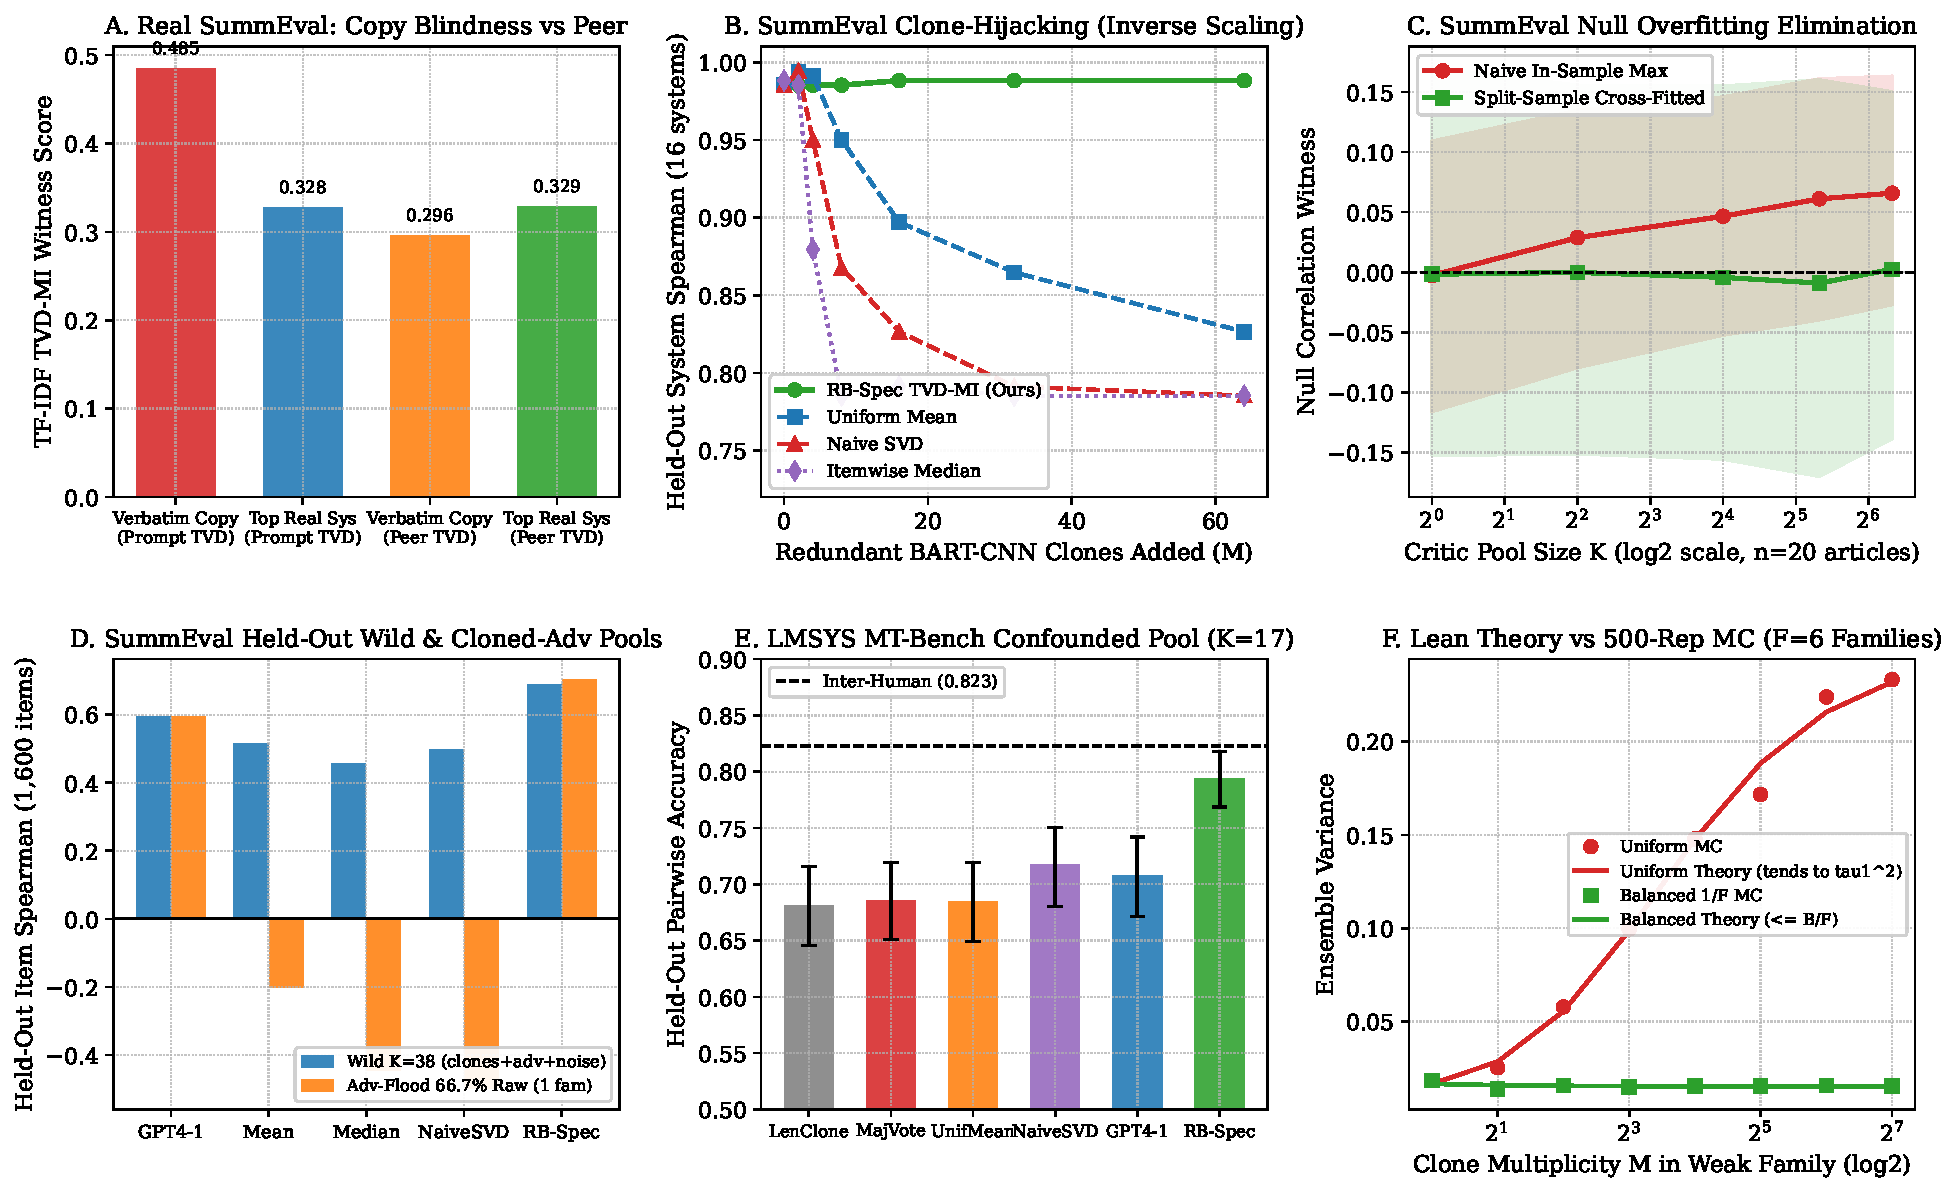
\includegraphics[width=\textwidth]{results/exp13_real_llm_and_theory_6panel.pdf}
\end{center}

\begin{table}[h]
\centering
\caption{\textbf{Held-out 5-fold CV summary on \textsc{SummEval} ($100$ articles, $1,600$ items; item Spearman across regimes) and \textsc{MT-Bench} ($80$ questions, $2,575$ decisive pairs); $95\%$ cluster-bootstrap CIs.}}
\resizebox{\textwidth}{!}{%
\begin{tabular}{@{}lccccc@{}}
\toprule
Method & \textsc{SummEval} Clean ($K=13$) & \textsc{SummEval} Wild ($K=38$) & \textsc{SummEval} Adv-Flood ($67\%$ raw) & Wild Mean Bias & \textsc{MT-Bench} Pair Acc. \\
\midrule
Single GPT-4 & $0.596\,[0.555,0.635]$ & $0.596\,[0.557,0.634]$ & $0.596\,[0.556,0.633]$ & $-0.476$ & $0.708\,[0.671,0.742]$ \\
Uniform Mean & $0.643\,[0.608,0.675]$ & $0.515\,[0.466,0.561]$ & $-0.201\,[-0.269,-0.131]$ & $-0.758$ & $0.685\,[0.649,0.720]$ \\
Itemwise Median & $0.483\,[0.429,0.535]$ & $0.457\,[0.398,0.513]$ & $-0.446\,[-0.505,-0.387]$ & $-0.523$ & $0.686\,[0.651,0.720]$ (Maj) \\
Naive SVD & $0.570\,[0.528,0.611]$ & $0.497\,[0.446,0.547]$ & $-0.500\,[-0.550,-0.450]$ & $-1.115$ & $0.718\,[0.681,0.751]$ \\
\textbf{\texttt{RB-Spec TVD-MI}} & $\mathbf{0.688\,[0.657,0.715]}$ & $\mathbf{0.689\,[0.659,0.718]}$ & $\mathbf{0.703\,[0.673,0.732]}$ & $-1.111$ & $\mathbf{0.795\,[0.769,0.820]}$ \\
\bottomrule
\end{tabular}}
\end{table}

\noindent\textbf{Sources.} Lean~4 proofs: \texttt{experiments/00\_\allowbreak lean\_\allowbreak formalization/\allowbreak lean/TvdmiJudge/NewTheory.lean}.
Python validation suite: \texttt{experiments/13\_\allowbreak ...\_\allowbreak 21Nov2026/\allowbreak run\_\allowbreak real\_\allowbreak llm\_\allowbreak and\_\allowbreak theory\_\allowbreak suite.py} and
\texttt{results/summary\_\allowbreak metrics.json}. Primary benchmarks: Fabbri et al.\ (TACL 2021, \textsc{SummEval}),
Liu et al.\ (EMNLP 2023, \textsc{G-Eval}), Zheng et al.\ (NeurIPS 2023, \textsc{MT-Bench}).
\end{document}
